\begin{pastexam}[label={px:ntust-110-ete-ds-03}]{臺科大電子所甲組 110 學年度 第 3 題}
（問答）

(10\%) Draw a binary tree that contains the letters: ``b'', ``u'', ``o'', ``s'', ``n'', such that
the inorder traversal spells ``bonus'' and the preorder traversal spells ``obuns''.
\end{pastexam}

\begin{pastsoln}
答案：
\begin{center}
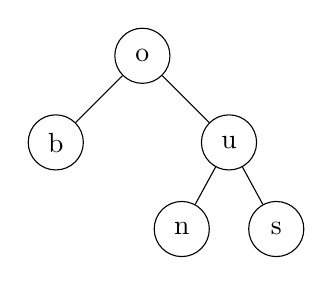
\begin{tikzpicture}[v/.style={draw,circle,minimum size=0.7cm,inner sep=0pt},
  level distance=1.1cm, level 1/.style={sibling distance=2.2cm},
  level 2/.style={sibling distance=1.2cm}]
\node[v] {o}
  child {node[v] {b}}
  child {node[v] {u}
    child {node[v] {n}}
    child {node[v] {s}}};
\end{tikzpicture}
\end{center}

做法（資結書第~7.4~節，前序加中序可以唯一決定二元樹）：前序的第一個字是根，在中序裡找到它，左邊
的字屬於左子樹、右邊的屬於右子樹；兩邊的字數也告訴我們前序要怎麼切。
\begin{enumerate}
\item 前序 \texttt{obuns} 的第一個字 \texttt{o} 是根。 中序 \texttt{bonus} 裡 \texttt{o} 的左邊是
\texttt{b}，右邊是 \texttt{nus}。 所以左子樹只有 \texttt{b}；右子樹的前序是前序裡接下來的
\texttt{uns}，中序是 \texttt{nus}。
\item 右子樹：前序 \texttt{uns} 的第一個字 \texttt{u} 是根。 中序 \texttt{nus} 裡 \texttt{u} 左邊是
\texttt{n}、右邊是 \texttt{s}，所以 \texttt{u} 的左子節點是 \texttt{n}，右子節點是 \texttt{s}。
\end{enumerate}
檢查：前序（根、左、右）是 o, b, u, n, s，拼成 obuns；中序（左、根、右）是 b, o, n, u, s，拼成
bonus，都符合。 因為前序加中序決定的樹是唯一的，這也是唯一的答案。
\end{pastsoln}
